% =====================================================================
%  Prabhavit Gupta - Tailored CV for BCG X
%  Target:   BCG X (Milan, Lombardy, Italy)
%  Role:     Visiting Forward Deployed AI Engineer (LinkedIn: 4388505837)
%  Compile:  tectonic cv/main_BCGX_VisitingForwardDeployedAIEngineer.tex OR pdflatex / lualatex
%  Needs:    photo.jpg in cv/
%  Rules:    ONE PAGE. 0 em-dashes. Plain voice. Clickable links.
% =====================================================================
\documentclass[a4paper,10pt]{article}

\usepackage[T1]{fontenc}
\usepackage[utf8]{inputenc}
\usepackage[top=0.70cm,bottom=0.70cm,left=1.0cm,right=1.0cm]{geometry}
\usepackage{titlesec}
\usepackage{enumitem}
\usepackage{hyperref}
\usepackage{xcolor}
\usepackage{graphicx}

\definecolor{accent}{HTML}{1F4E78}
\hypersetup{colorlinks=true, urlcolor=accent, linkcolor=accent}
\pagestyle{empty}
\setlength{\parindent}{0pt}

\titleformat{\section}{\large\bfseries\color{accent}}{}{0em}{}[\vspace{-0.6em}\rule{\textwidth}{0.8pt}]
\titlespacing{\section}{0pt}{2pt}{1pt}

\newcommand{\role}[4]{%
  \textbf{#1} \hfill \textbf{#2}\\[1pt]%
  \textit{#3} \hfill \textit{#4}\\[2pt]%
}
\setlist[itemize]{leftmargin=1.2em, itemsep=0pt, topsep=1pt, parsep=0pt}

\begin{document}

% ================= HEADER =================
\begin{minipage}[c]{0.80\textwidth}
  {\Huge\bfseries Prabhavit Gupta}\\[3pt]
  {\color{accent}\large Visiting Forward Deployed AI Engineer: LLM Systems, Enterprise APIs \& Delivery}\\[5pt]
  {\footnotesize +39 351 610 7807 ~$\vert$~
  \href{mailto:prabhavitg@gmail.com}{prabhavitg@gmail.com} ~$\vert$~
  \href{https://www.linkedin.com/in/prabhavit/}{linkedin.com/in/prabhavit} ~$\vert$~
  \href{https://github.com/prab-gupta}{github.com/prab-gupta} ~$\vert$~
  Venice, Italy (Hybrid Milan / Relocation)}
\end{minipage}\hfill
\begin{minipage}[c]{0.18\textwidth}
  \raggedleft\IfFileExists{photo.jpg}{\includegraphics[width=2.0cm]{photo.jpg}}{\IfFileExists{cv/photo.jpg}{\includegraphics[width=2.0cm]{cv/photo.jpg}}{}}
\end{minipage}
\vspace{-2pt}

% ================= SUMMARY =================
\section{Summary}
Forward deployed AI engineer who bridges client problem discovery, rapid software prototyping, and enterprise-grade AI deployment. Experienced in embedding directly with product teams to build agentic workflows, multi-format RAG ingestion engines, and governed human-in-the-loop validation systems. At FlowSpace, architected an automated document extraction pipeline (900+ listings drafted), deployed live customer-facing support agents with confidence-based escalation, and led the platform migration off a legacy stack to Next.js and Laravel (scaling 2,000 to 4,500+ users). Daily practitioner with Claude Code, TypeScript, Python, REST APIs, and event-driven architectures.

% ================= SKILLS =================
\section{Skills}
\begin{itemize}
  \item \textbf{Forward Deployed \& Solutions Engineering:} Client discovery, technical scoping, rapid prototyping, production rollouts, human-in-the-loop review interfaces, non-technical stakeholder enablement, field troubleshooting, product feedback loops
  \item \textbf{Agentic AI \& LLM Systems:} Claude Code (daily driver), Anthropic Claude API, OpenAI API, prompt engineering, Model Context Protocol (MCP), tool use and function calling, structured JSON output validation, RAG architectures, multi-agent orchestration, confidence scoring, evaluation harnesses
  \item \textbf{Full-Stack, APIs \& Architecture:} TypeScript, Python, Node.js, Next.js, Laravel (PHP), REST APIs, OpenAPI, webhooks, asynchronous jobs, retry and rate-limit handling, PostgreSQL, Supabase, third-party integrations (OfficeRnD, Nexudus, CRM, Google APIs)
  \item \textbf{Testing, Reliability \& DevOps:} Docker, Git/GitHub, CI/CD, Playwright automated testing, Postman contract testing, unit testing, schema enforcement, logging, exception escalation, production monitoring
\end{itemize}

% ================= EXPERIENCE =================
\section{Experience}

\role{\href{https://flowspace.co}{FlowSpace.co}}{Mar 2024 - Aug 2026}{Lead Developer \& AI Engineer (Full-time, Freelance)}{London, UK (remote)}
\begin{itemize}
  \item Architected and deployed an end-to-end multi-format AI document ingestion pipeline (n8n, Claude API, TypeScript) with tool use and structured parsing to extract data from unstructured PDFs, spreadsheets, and web sources into validated schemas; drafted 900+ production listings.
  \item Designed governed agentic workflows with strict schema validation and approval gates, enabling non-technical staff and consultants to safely review and verify AI outputs prior to production release.
  \item Built and deployed customer-facing support AI agents querying live operational databases with confidence scoring thresholds and deterministic fallback paths to human staff.
  \item Engineered bidirectional enterprise integrations with OfficeRnD and Nexudus APIs for automated bookings, managing rate limits, webhooks, and retry logic across service boundaries.
  \item Led core platform migration off a legacy stack to coded Next.js and Laravel (PostgreSQL), scaling active users from 2,000 to 4,500+ without downtime.
\end{itemize}

\role{\href{https://get2germany.com}{Get2Germany.com}}{Jan 2024 - May 2024}{Developer \& Automation Specialist (Part-time)}{Berlin, Germany (remote)}
Built automated data collection and validation pipelines using n8n and Google APIs, streamlining database synchronization and candidate matching logic.\\[1pt]

\role{\href{https://clubee.com}{Clubee.com}}{Sep 2023 - Aug 2024}{Developer \& QA (Full-time, Freelance)}{Foetz, Luxembourg (remote)}
Integrated core REST APIs across frontend modules, executed QA/unit testing, and delivered administrative federation dashboards.\\[1pt]

\role{\href{https://tractionboard.co}{Tractionboard.co}}{Aug 2023 - Oct 2023}{Developer (Internship)}{Utrecht, Netherlands (remote)}
Integrated OpenAI/ChatGPT and Sendgrid APIs, designed responsive frontend interfaces, and debugged production features.

% ================= PROJECTS =================
\section{Selected Projects}
\begin{itemize}
  \item \textbf{\href{https://github.com/prab-gupta/llm-doc-parser}{LLM Document Parser}} (\href{https://github.com/prab-gupta/llm-doc-parser}{github.com/prab-gupta/llm-doc-parser}): Open-source engine demonstrating multi-format document parsing (PDF, image, text) into strictly typed, validated JSON structures with automated error recovery.
  \item \textbf{\href{https://smarturlink.com/}{Urlink}} (2025): Project Manager \& Integration Developer; managed client requirements, platform logic, and automated workflows using Next.js and Supabase.
  \item \textbf{\href{https://ultrastrategy.com}{UltraStrategy}} (2024 - 2025): AI Automation Developer; built an LLM document extraction tool with n8n and Eden AI for multi-profile candidate data processing.
\end{itemize}

% ================= EDUCATION & CERTIFICATIONS =================
\section{Education \& Certifications}
\textbf{Ca' Foscari University of Venice} \hfill Oct 2020 - Jun 2024\\
BA Philosophy, International Studies \& Economics (Minor: Entrepreneurship)\\[1pt]
\textbf{Certifications:} Microsoft Copilot Studio Agent Academy \textbullet\ Microsoft: Introduction to building AI agents \textbullet\ Microsoft Power Automate \textbullet\ Tray.AI Build Practitioner (Sep 2024)

% ================= WORK AUTHORIZATION =================
\vspace{2pt}
{\small \textbf{Work authorization:} Italian EU Long Term Residence Permit (unrestricted EU work rights, no visa sponsorship needed in Italy/EU); available immediately. \quad \textbf{Languages:} English (fluent C2), Hindi (native), Italian (conversational).}

\end{document}